\documentclass{article}
\usepackage[margin=1in]{geometry}
\usepackage[nodisplayskipstretch]{setspace}
\usepackage{amsmath, nccmath, bm}
\usepackage{amssymb}
\usepackage{enumitem}
\usepackage{graphicx}
\usepackage{float}
\usepackage{listings}
\usepackage{hyperref}
\usepackage[svgnames]{xcolor}
\usepackage{indentfirst}
%\usepackage{chngcntr}
%\counterwithin{table}{section}
\graphicspath{
{./images}}

%\hypersetup{
%    colorlinks=true,
%    linkcolor=black,
%    filecolor=black,      
%    urlcolor=blue
%    }

\newcommand{\zerodisplayskip}{
	\setlength{\abovedisplayskip}{0pt}%
	\setlength{\belowdisplayskip}{0pt}%
	\setlength{\abovedisplayshortskip}{0pt}%
	\setlength{\belowdisplayshortskip}{0pt}%
	\setlength{\mathindent}{0pt}}
	
\definecolor{vgreen}{RGB}{104,180,104}
\definecolor{vblue}{RGB}{49,49,255}
\definecolor{vorange}{RGB}{255,143,102}

\lstdefinestyle{verilog-style}
{
    language=Verilog,
    basicstyle=\small\ttfamily,
    keywordstyle=\color{vblue},
    identifierstyle=\color{black},
    commentstyle=\color{vgreen},
    numbers=left,
    numberstyle=\tiny\color{black},
    numbersep=10pt,
    tabsize=8,
    moredelim=*[s][\colorIndex]{[}{]},
    literate=*{:}{:}1
}

\lstset{style={verilog-style},showstringspaces=false}

\lstdefinestyle{nocoloring}{
    keywordstyle=\color{black},
    commentstyle=\color{black},
    stringstyle=\color{black}
}

\makeatletter
\newcommand*\@lbracket{[}
\newcommand*\@rbracket{]}
\newcommand*\@colon{:}
\newcommand*\colorIndex{%
    \edef\@temp{\the\lst@token}%
    \ifx\@temp\@lbracket \color{black}%
    \else\ifx\@temp\@rbracket \color{black}%
    \else\ifx\@temp\@colon \color{black}%
    \else \color{vorange}%
    \fi\fi\fi
}
\makeatother

\newcommand{\code}[1]{%
	\colorbox{Gainsboro}{\texttt{#1}}%
}

\title{Lab 3}
\author{Owen Sowatzke}
\date{April 21, 2025}

\begin{document}

	% \offinterlineskip
	% \setlength{\lineskip}{12pt}
	% \zerodisplayskip
	\maketitle
	
	\section{Introduction}
	
	In this lab, we perform design and verification for an ARM 8-bit microprocessor. We start by simulating a SystemVerilog model of the microprocessor in NC verilog. Then, we design 8-bit AND and OR wordslices in Cadence Virtuoso. For each of these wordslices, we create a schematic, symbol, and layout. Then, we incorporate each of our wordslices into the ALU schematic and layout. Similarly, we update the datapath layout with our updated ALU. At each stage of the design, we verify our layouts using DRC and LVS. Finally, we create a netlist from our design and validate its behavior in simulation. 
	
	\section{AND Wordslice}
	\label{section::and_wordslice}
	
	In this section, we perform design and verification of our AND wordslice. Our wordslice specifically contains 8 \texttt{and2\_1x} gates from the \texttt{muddlib11} library. The resulting schematic is shown in Figure \ref{fig::and2_1x_8_schematic}. Note the vectorized ports and component instances.
	
	\begin{figure}[H]
		\centerline{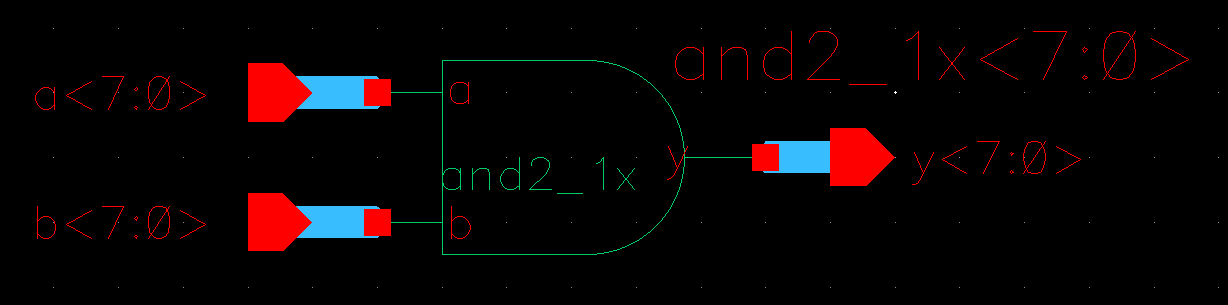
\includegraphics[width=0.5\textwidth]{and2_1x_8_schematic.png}}
		\caption{Schematic for AND Wordslice}
		\label{fig::and2_1x_8_schematic}
	\end{figure}
	
	\noindent Next, we create a symbol for our AND wordslice. For this step, we start with a copy of the \texttt{and2\_1x} symbol and make small incremental updates. Our wordslice symbol with these updates is shown in Figure \ref{fig::and2_1x_8_symbol}. Note that the port names and wire widths have been updated to reflect the vectorized inputs and outputs.
	
	\begin{figure}[H]
		\centerline{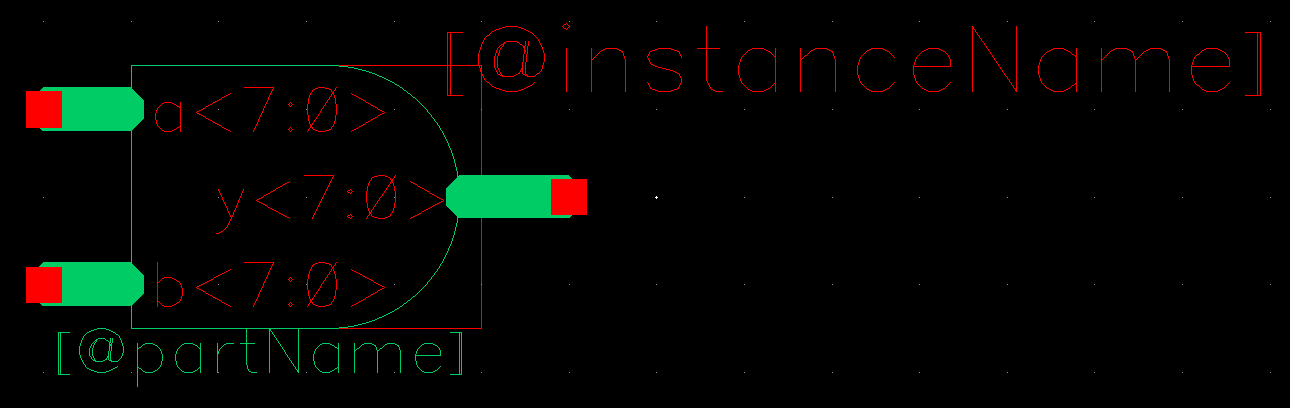
\includegraphics[width=0.5\textwidth]{and2_1x_8_symbol.png}}
		\caption{Symbol for AND Wordslice}
		\label{fig::and2_1x_8_symbol}
	\end{figure}
	
	\noindent Then, we create a layout for our wordslice. For the layout, we use an $8 \times 1$ mosiac of AND gates. The resulting layout with different display levels is shown in Figures \ref{fig::and2_1x_8_layout_mosiac_overview} and \ref{fig::and2_1x_8_layout_detailed}. Note that the our images are rotated $90^{\circ}$ with respect to the layouts.  
	
	\begin{figure}[H]
		\centerline{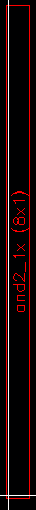
\includegraphics[height=0.8\textwidth, angle=270]{and2_1x_8_layout_mosiac_overview.png}}
		\caption{AND Gate Mosiac Layout Display Level = 0}
		\label{fig::and2_1x_8_layout_mosiac_overview}
	\end{figure}
	
	\begin{figure}[H]
		\centerline{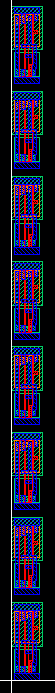
\includegraphics[height=0.8\textwidth, angle=270]{and2_1x_8_layout_detailed.png}}
		\caption{AND Gate Mosiac Layout Display Level = 1}
		\label{fig::and2_1x_8_layout_detailed}
	\end{figure}
	
	\noindent After placing the AND gates, we placed input and output ports for each gate. However, virtuoso shorted each element of the input/output buses. These shorts are displayed on an individual AND gates in Figure \ref{fig::and2_1x_8_cell_with_shorts} and in the Annotation Browser in Figure \ref{fig::and2_1x_8_annotation_shorts}. 
	
	\begin{figure}[H]
		\centerline{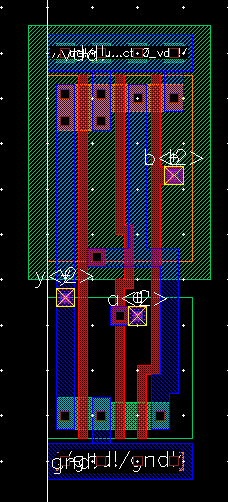
\includegraphics[width=0.2\textwidth]{and2_1x_8_cell_with_shorts.png}}
		\caption{Shorts Marked in the Schematic}
		\label{fig::and2_1x_8_cell_with_shorts}
	\end{figure}
	
	\begin{figure}[H]
		\centerline{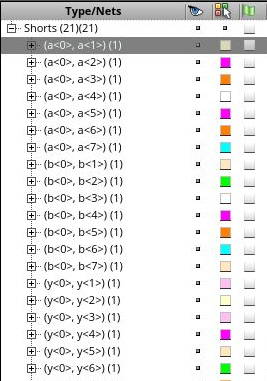
\includegraphics[width=0.35\textwidth]{and2_1x_8_annotation_shorts.png}}
		\caption{Shorts Called Out by the Annotation Browser}
		\label{fig::and2_1x_8_annotation_shorts}
	\end{figure}
	
	\noindent To work around this, I instantiated a single AND gate and then copied it 7 times with $33{\mu}m$ spacing. The resulting schematic at display level = 0 is shown in Figure \ref{fig::and2_1x_8_layout_overview}. Note that the AND gates are now displayed individually at this display level. However, the underlying content is the same.
	
	\begin{figure}[H]
		\centerline{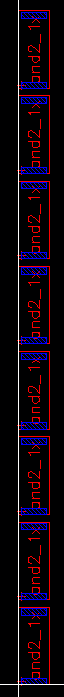
\includegraphics[height=0.8\textwidth, angle=270]{and2_1x_8_layout_overview.png}}
		\caption{AND Wordslice Created without Mosiac at Display Level = 0}
		\label{fig::and2_1x_8_layout_overview}
	\end{figure}
	
	\noindent For better visualization, we also highlight the port placement for a single AND gate, which is shown in Figure \ref{fig::and2_1x_8_single_gate_ports}.
	
	\begin{figure}[H]
		\centerline{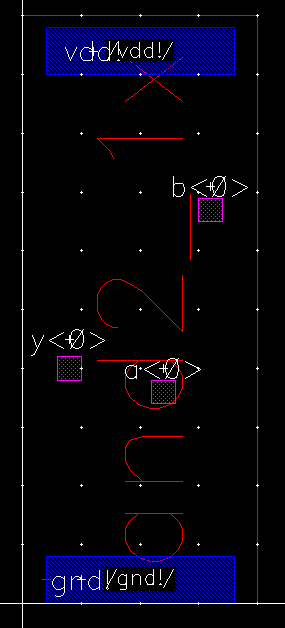
\includegraphics[width=0.25\textwidth]{and2_1x_8_single_gate_ports.png}}
		\caption{Port Placement for a Given AND Gate}
		\label{fig::and2_1x_8_single_gate_ports}
	\end{figure}
	
	\noident Next, we performed DRC and LVS for our layout. According to the Cadence Virtuoso IC23.1 documentation, we should have been able to do this with Verify \textgreater\ DRC and Verify \textgreater\ LVS. However, the Verify drop-down menu did not include these options. The drop-down menu from our Virtuoso installation is shown in Figure \ref{fig::verify_dropdown_menu}, and the expected menu is shown in Figure \ref{fig::verify_dropdown_menu_doc}.
	
	\begin{figure}[H]
		\centerline{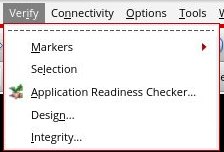
\includegraphics[width=0.4\textwidth]{verify_dropdown_menu.png}}
		\caption{Verify Drop-Down Menu in Layout Window}
		\label{fig::verify_dropdown_menu}
	\end{figure}
	
	\begin{figure}[H]
		\centerline{\fbox{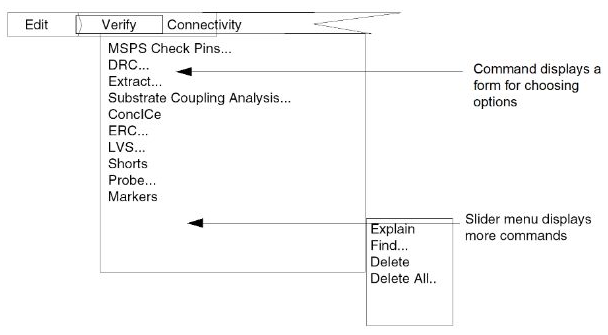
\includegraphics[height=0.4\textwidth]{verify_dropdown_menu_doc.png}}}
		\caption{Verify Drop-Down Menu per Documentation}
		\label{fig::verify_dropdown_menu_doc}
	\end{figure}
	
	\noindent Luckily, we were able to perform comparable analysis using Verify \textgreater\ Design... and Verify \textgreater\ Application Readiness Checker...
	
	% , likely because of a bad installation or bad environment. 
	% As a result, I settled for a reduced set of checks.
	
	\noindent Instead, I performed a reduced set of checks using Verify \textgreater\ Application Readiness Checker.... To get passing results I had to do two things. First, I had to associate each of the AND gates in the schematic with gates in my layout using Connectivity \textgreater\ Define Device Correspondence. Second, I had to create "Must Connect" groups for gnd! and vdd!, which I did with Pins \textgreater\ Pin Connectivity Setting.... My final application readiness checks are shown in Figure \ref{fig::and_application_readiness_check}.
	
	\begin{figure}[H]
		\centerline{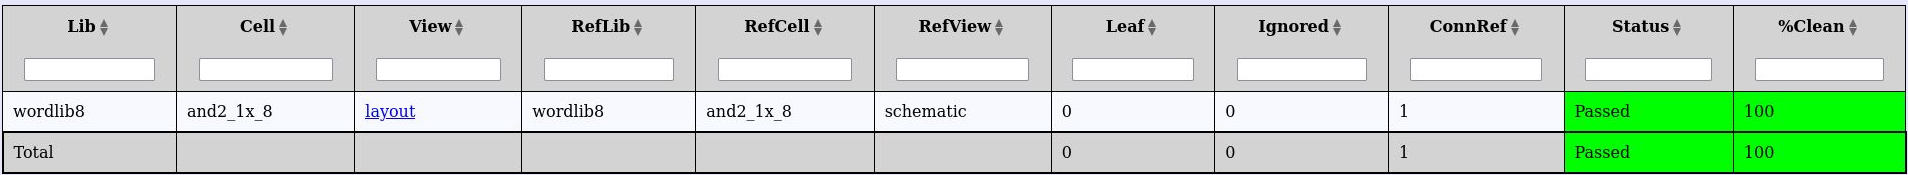
\includegraphics[width=0.9\textwidth]{and_application_readiness_check.png}}
		\caption{Application Readiness Check Results}
		\label{fig::and_application_readiness_check}
	\end{figure}
	
	\noindent I also was able to use Verify \textgreater\ Design to populate the DRC annotations in the annotation browser. These annotations are shown in Figure \ref{fig::and_drc} and confirm no DRC failures.
	
	\begin{figure}[H]
		\centerline{\fbox{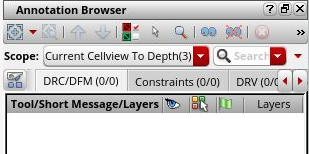
\includegraphics[width=0.5\textwidth]{and_drc.png}}}
		\caption{DRC Annotations Showing All Checks Passing}
		\label{fig::and_drc}
	\end{figure}
	
	\section{OR Wordslice}
	
	We repeat the process given in Section \ref{section::and_wordslice} to create an OR wordslice.  Our wordslice specifically contains 8 \texttt{or2\_1x} gates from the \texttt{muddlib11} library. The resulting schematic is shown in Figure \ref{fig::or2_1x_8_schematic}. Note the vectorized ports and component instances.
	
	\begin{figure}[H]
		\centerline{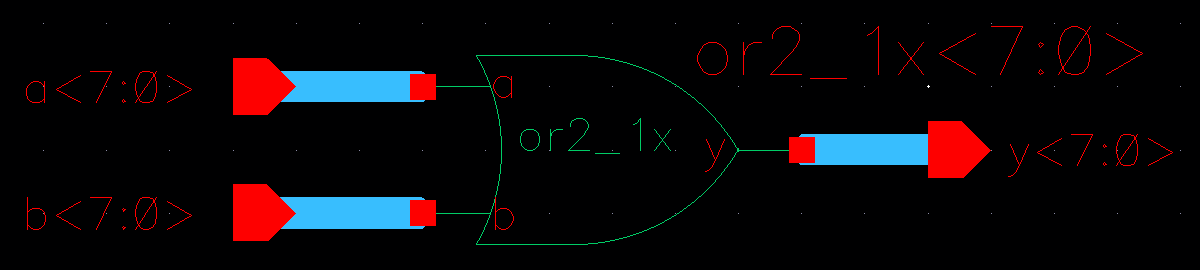
\includegraphics[width=0.5\textwidth]{or2_1x_8_schematic.png}}
		\caption{Schematic for OR Wordslice}
		\label{fig::or2_1x_8_schematic}
	\end{figure}
	
	\noindent Next, we create a symbol for our OR wordslice. For this step, we start with a copy of the \texttt{or2\_1x} symbol and make small incremental updates. Our wordslice symbol with these updates is shown in Figure \ref{fig::or2_1x_8_symbol}. Note that the port names and wire widths have been updated to reflect the vectorized inputs and outputs.
	
	\begin{figure}[H]
		\centerline{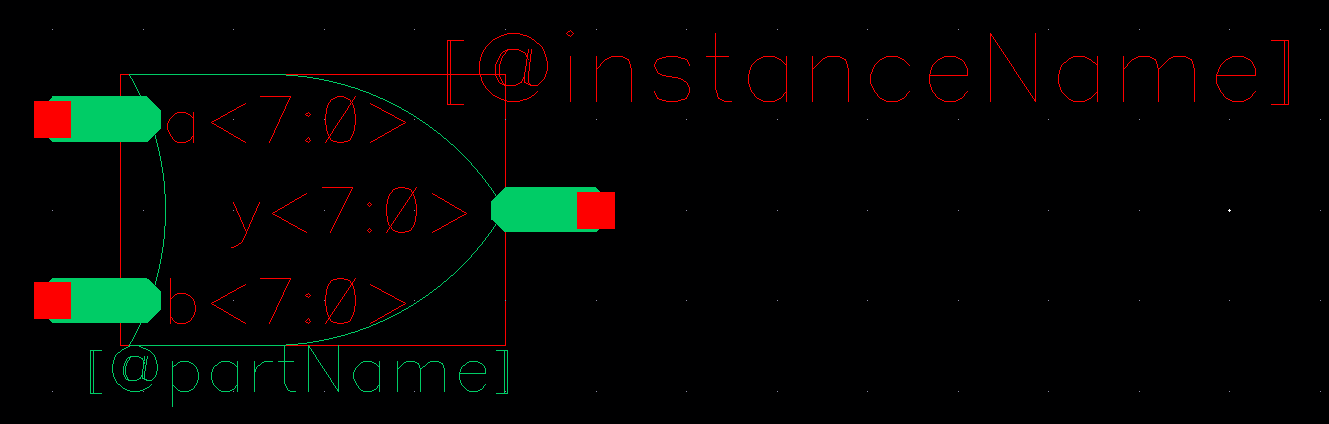
\includegraphics[width=0.5\textwidth]{or2_1x_8_symbol.png}}
		\caption{Symbol for OR Wordslice}
		\label{fig::or2_1x_8_symbol}
	\end{figure}
	
	\noindent Then, we create a layout for our wordslice. We leverage what we learned from the previous section and copy OR gates instead of using a mosiac. This helps us to prevent unintentional shorts. The layout with different display levels is shown in Figures \ref{fig::or2_1x_8_layout_overview} and \ref{fig::or2_1x_8_layout_detailed}.
	
	\begin{figure}[H]
		\centerline{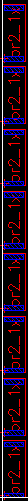
\includegraphics[height=0.8\textwidth, angle=270]{or2_1x_8_layout_overview.png}}
		\caption{OR Wordslice Layout Display Level = 0}
		\label{fig::or2_1x_8_layout_overview}
	\end{figure}
	
	\begin{figure}[H]
		\centerline{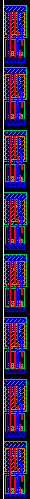
\includegraphics[height=0.8\textwidth, angle=270]{or2_1x_8_layout_detailed.png}}
		\caption{OR Wordslice Layout Display Level = 1}
		\label{fig::or2_1x_8_layout_detailed}
	\end{figure}
	
	\noindent We also highlight the port placement for a single OR gate, which is shown in Figure \ref{fig::or2_1x_8_single_gate_ports}.
	
	\begin{figure}[H]
		\centerline{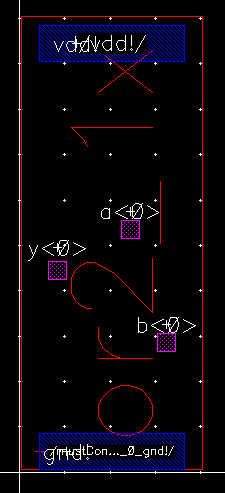
\includegraphics[width=0.25\textwidth]{or2_1x_8_single_gate_ports.png}}
		\caption{Port Placement for a Given OR Gate}
		\label{fig::or2_1x_8_single_gate_ports}
	\end{figure}
	
	\noindent Next, following the work from the previous section, we perform application readiness checks and check the annotations browser for DRC failures. To avoid errors in the application readiness checks, we map gates in the schematic to gates in the layout and create "Must Connect" groups for gnd! and vdd! The application readiness checks shown in Figure \ref{fig::or_application_readiness_check} and DRC checks shown in Figure \ref{fig::or_drc} show no errors.
	
	\begin{figure}[H]
		\centerline{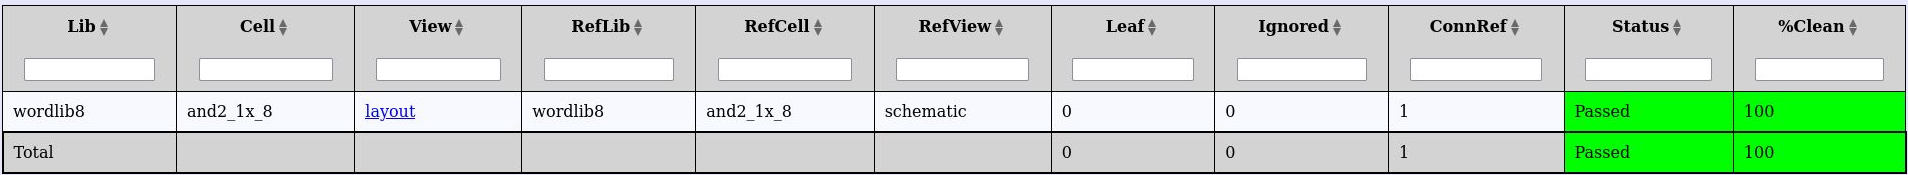
\includegraphics[width=0.9\textwidth]{and_application_readiness_check.png}}
		\caption{Application Readiness Check Results}
		\label{fig::or_application_readiness_check}
	\end{figure}
	
	\begin{figure}[H]
		\centerline{\fbox{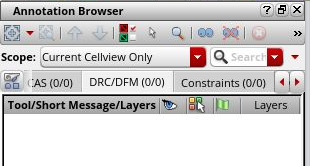
\includegraphics[width=0.5\textwidth]{or_drc.png}}}
		\caption{DRC Annotations Showing All Checks Passing}
		\label{fig::or_drc}
	\end{figure}
	
	\section{ALU}
	
	In this section, we complete the ALU schematic using the AND and OR wordslices we created in the previous sections. The resulting schematic is shown in Figure \ref{fig::alu_schematic}.
	
	\begin{figure}[H]
		\centerline{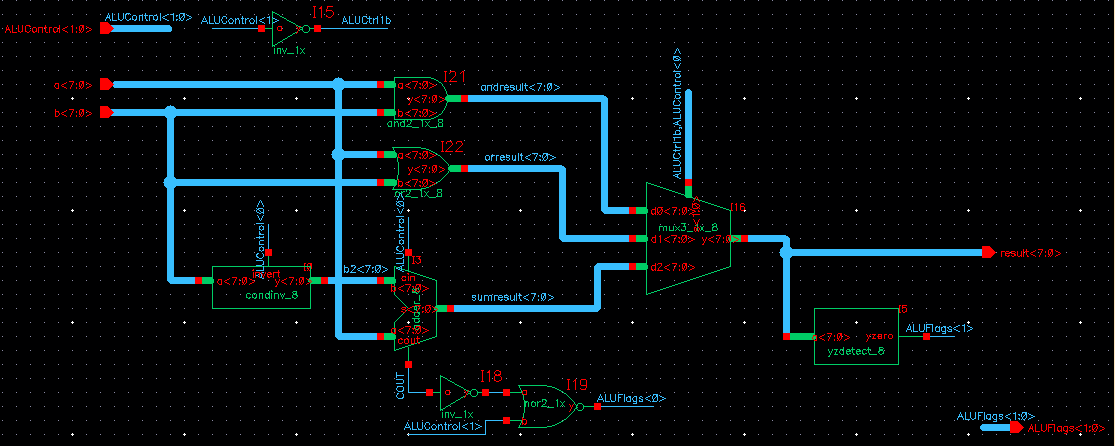
\includegraphics[width=0.9\textwidth]{alu_schematic.png}}
		\caption{ALU Schematic after Adding AND and OR Wordslices}
		\label{fig::alu_schematic}
	\end{figure}
	
	\noindent Then, we modify the ALU layout to include the AND and OR wordslices. The layout with different display levels is shown in Figures \ref{fig::alu_layout_overview} and \ref{fig::alu_layout_detailed}. The AND wordslice (top) and OR wordslice (bottom) are highlighted in both of the layouts. Before rotation, the AND gate is on the left and the OR gate is on the right.
	
	\begin{figure}[H]
		\centerline{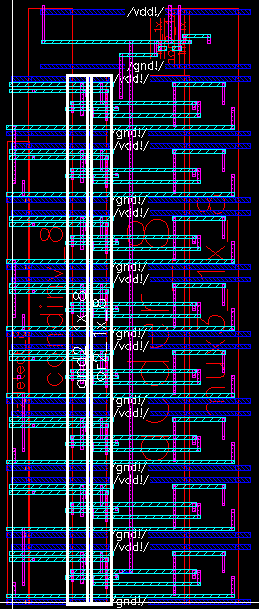
\includegraphics[height=0.8\textwidth, angle=270]{alu_layout_overview.png}}
		\caption{ALU Layout Display Level = 0}
		\label{fig::alu_layout_overview}
	\end{figure}
	
	\begin{figure}[H]
		\centerline{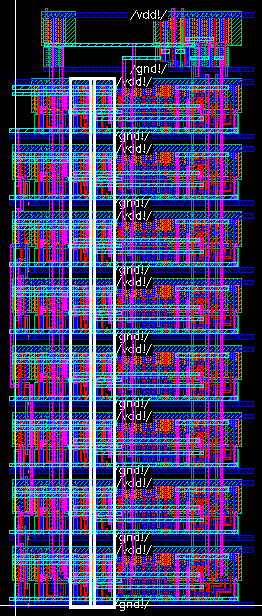
\includegraphics[height=0.8\textwidth, angle=270]{alu_layout_detailed.png}}
		\caption{ALU Layout Display Level = 1}
		\label{fig::alu_layout_detailed}
	\end{figure}
	
	\noindent We focus on the layout for the first bit of the ALU datapath in Figure \ref{fig::alu_layout_bit0}. The AND and OR wordslices are highlighted in the figure. The AND wordslice is on the left, and the OR wordslice is on the right. Examining the layout, we see that the inputs of both gates are correctly connected to the \texttt{a} and \texttt{b} bitlines. Additionally, we see that the output of the AND gate is connected to \texttt{d0}, while the output of the OR gate is connected to \texttt{d1}. This is consistent with our schematic shown in Figure \ref{fig::alu_schematic}.
	
	\begin{figure}[H]
		\centerline{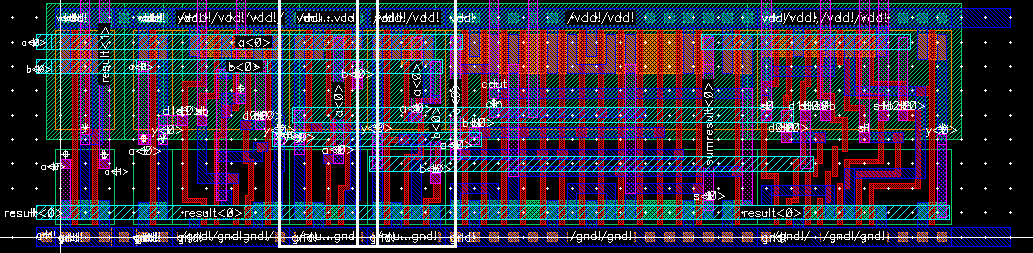
\includegraphics[width=0.8\textwidth]{alu_layout_bit0.png}}
		\caption{Layout for the First Bit of the ALU Datapath}
		\label{fig::alu_layout_bit0}
	\end{figure}
	
	\noindent Because the DRC and LVS checks dropdowns are missing, we perform an applications readiness check and look for DRC errors in the annotation browser. The application readiness check is shown in Figure \ref{fig::alu_application_readiness_check} and the DRC annotations are shown in Figure \ref{fig::alu_drc}.
	
	\begin{figure}[H]
		\centerline{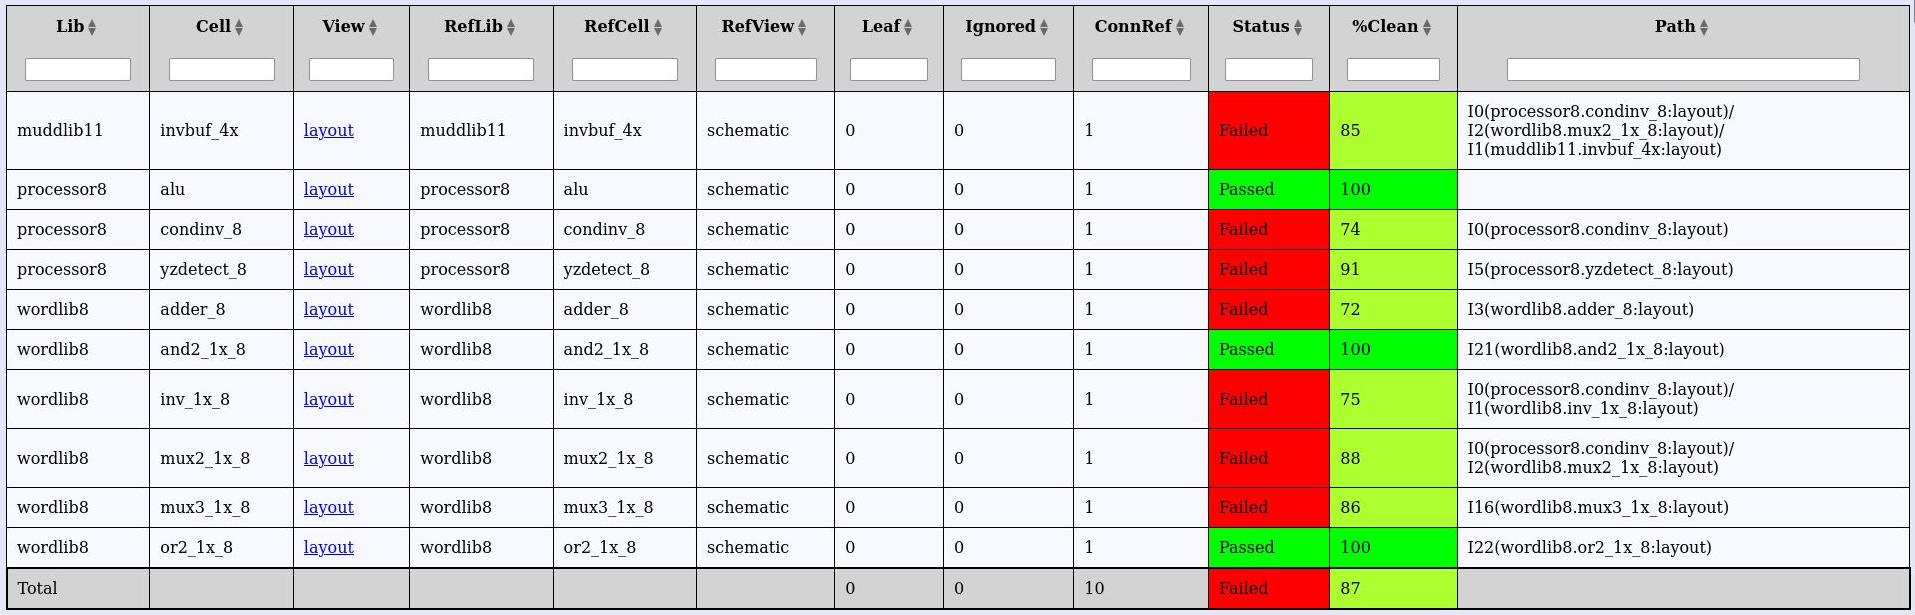
\includegraphics[width=0.9\textwidth]{alu_application_readiness_check.png}}
		\caption{Application Readiness Check for ALU}
		\label{fig::alu_application_readiness_check}
	\end{figure}
	
	\begin{figure}[H]
		\centerline{\fbox{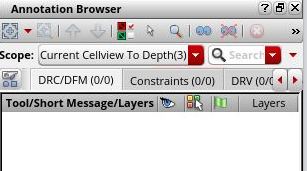
\includegraphics[width=0.5\textwidth]{alu_drc.png}}}
		\caption{DRC Annotations Showing All Checks Passing}
		\label{fig::alu_drc}
	\end{figure}
	
	\noindent Unlike our previous runs, the application readiness checks include failures. However, these failures are not in the AND slice, OR slice, or ALU, so we consider them out of scope for this lab. Additionally, these failures do not result in any DRC errors and they do not preclude us from getting passing LVS results.
	
	\section{Datapath}
	
	In this section, we perform DRC and LVS checks for the datapath schematic with the updated ALU. We also show the schematic for the datapath in Figure \ref{fig::datapath_schematic}. However, we don't need to make any edits to the schematic since the ALU block is already included and its ports are unchanged.
	
	\begin{figure}[H]
		\centerline{\fbox{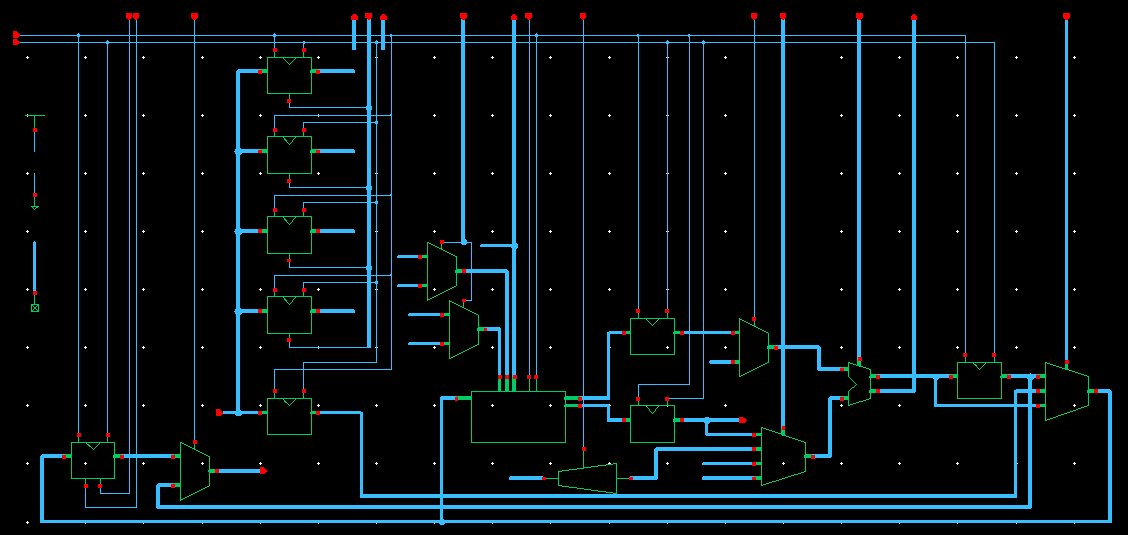
\includegraphics[width=0.9\textwidth]{datapath_schematic.png}}}
		\caption{Datapath Schematic}
		\label{fig::datapath_schematic}
	\end{figure}
	
	\noindent Next, we show the layout of the datapath in Figure \ref{fig::datapath_layout}.
	
	\begin{figure}[H]
		\centerline{\fbox{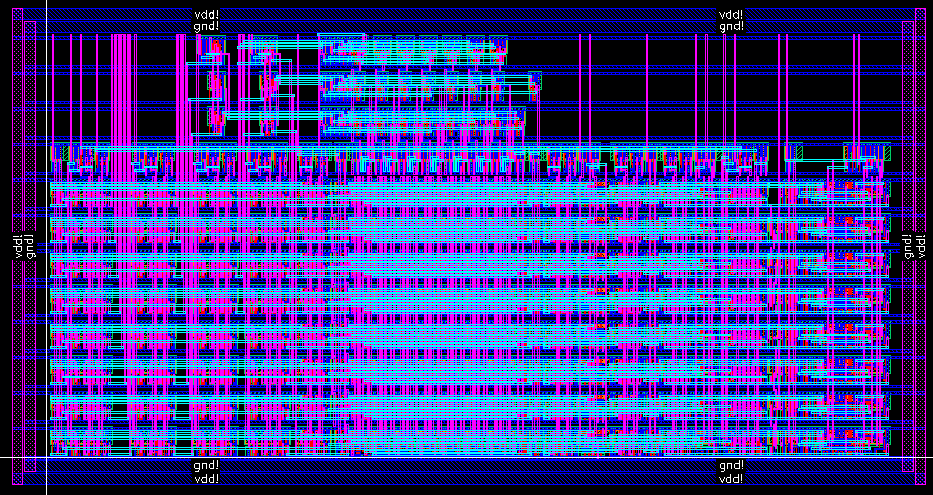
\includegraphics[width=0.9\textwidth]{datapath_layout.png}}}
		\caption{Datapath Layout}
		\label{fig::datapath_layout}
	\end{figure}
	
	\noindent Note that layout automatically pulls the updates from the ALU layout. However, we still need to perform DRC and LVS checks to validate the overall design. Due to shortcomings with the tool, we are again limited to application readiness checks and a review of the DRC annotations. The application readiness checks are included in Figure \ref{fig::datapath_application_readiness_check}, and the DRC annotations are shown in Figure \ref{fig::datapath_drc}.
	
	\begin{figure}[H]
		\centerline{\fbox{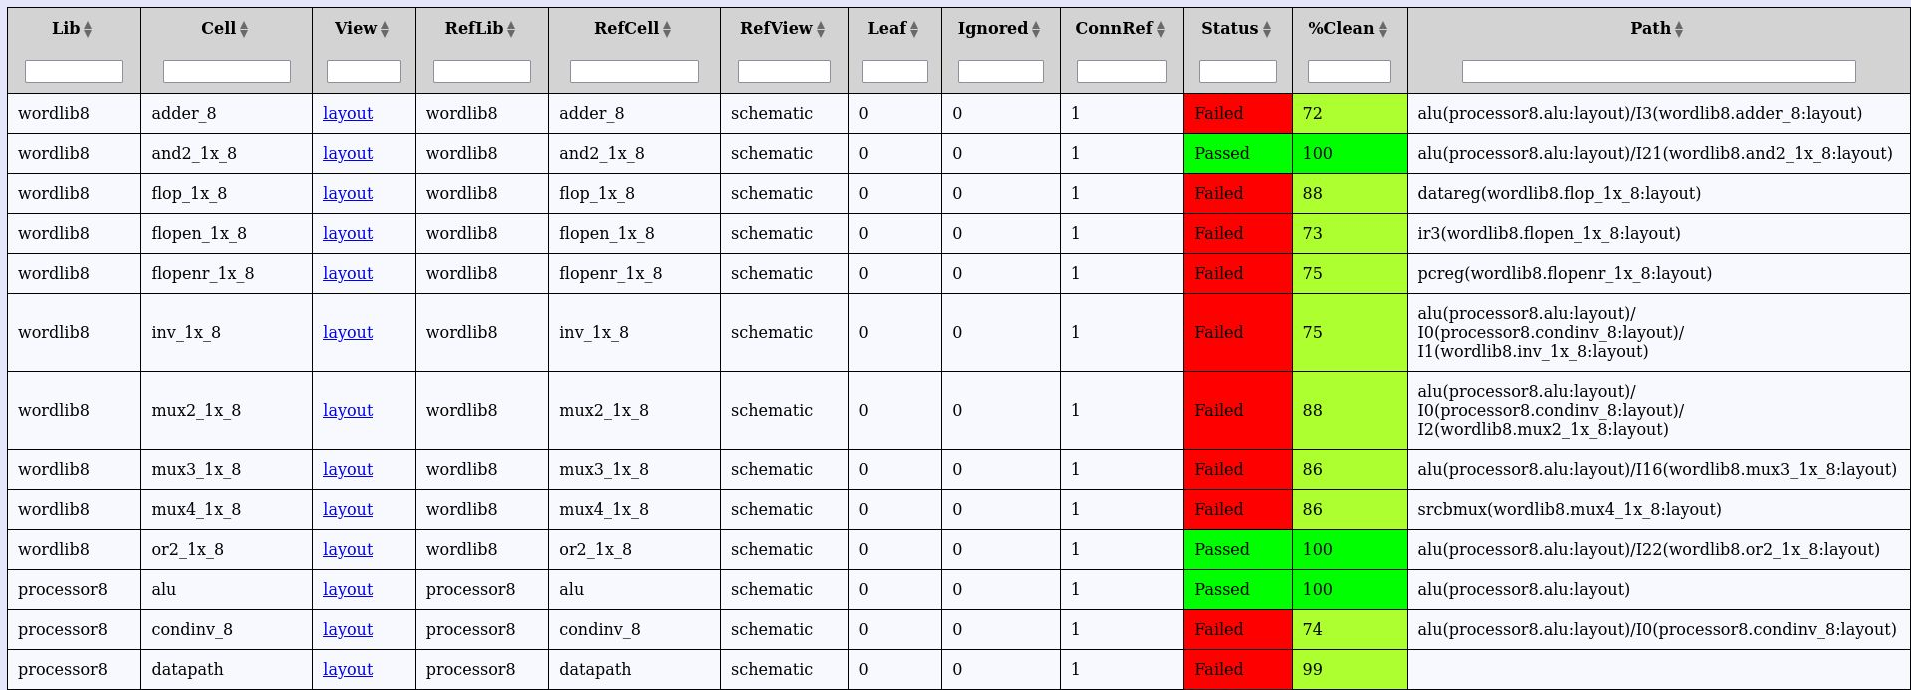
\includegraphics[width=0.9\textwidth]{datapath_application_readiness_check.png}}}
		\caption{Application Readiness Check for Datapath (Additional Blocks Not Shown)}
		\label{fig::datapath_application_readiness_check}
	\end{figure}
	
	\begin{figure}[H]
		\centerline{\fbox{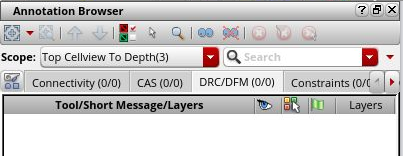
\includegraphics[width=0.5\textwidth]{datapath_drc.png}}}
		\caption{DRC Annotations Showing All Checks Passing}
		\label{fig::datapath_drc}
	\end{figure}
	
	\noindent Once again, we are more interested in the DRC results than the application readiness checks. However, we note that the application readiness checks pass for the AND wordslice, OR wordslice, and ALU.
	
	\section{Conclusion}
	
	In this lab, we performed design and verification for an ARM 8-bit microprocessor. We attempted to simulate a SystemVerilog model of the microprocessor in NC verilog. However, due to the IT configuration of the session server, we were unable to perform this simulation. We also designed 8-bit AND and OR wordslices in Cadence Virtuoso. For each of these wordslices, we created a schematic, symbol, and layout. While creating the layout, we ran into problems with the mosiac command creating uintentional short circuits. We were able to work around this by creating multiple copies of the same cell. We ran into additional errors performing DRC and LVS. As a result, we resorted to application readiness checks and DRC annotations to verify our design. Both these checks passed without issues for our AND and OR wordslices. 
	
	Once our wordslices were validated, we incorporated them into the ALU and updated the schematic and layout. We also performed application readiness checks and DRC annotations on this design. We failed some of the application readiness checks on modules we did not edit. We ignored these checks for the lab. Luckily, our DRC passed, which we considered a more meaningful metric. The application readiness checks also do not preclude us from passing LVS checks once the tools were properly configured. Finally, we updated the layouts and schematics for the datapath and attempted to generate a netlist. Unfortunately, another IT issue prevented us from fully generating the netlist. However, with a proper tool and environment, we believe the rest of the items in this lab can be completed.
	
\end{document}